\documentclass[11pt, a4paper, oneside, openright]{book} %draft

\usepackage{graphicx,color}
\usepackage{amssymb, amsmath, array}
\usepackage{listings}


\newtheorem{dfn}{Definition}



\begin{document}

% Example of title page for the projects carried out within the lasec 

% Simply include it in your mastex tex file: 
%        % Example of title page for the projects carried out within the lasec 

% Simply include it in your mastex tex file: 
%        % Example of title page for the projects carried out within the lasec 

% Simply include it in your mastex tex file: 
%        \input{cover}


% Updated March 2006 (SP)


\newcommand{\logoepfl}[0]{
  \begin{center}
    
\includegraphics[width=4cm]{logo_epfl_coul.eps}
  \end{center}
  \vspace{0.3cm}
  \hrule
}
\newcommand{\logolasec}[0]{
  \vspace{1cm}
  \hrule
  \begin{center}
    
\includegraphics[width=4.5cm]{logo_lasec_coul.eps}
  \end{center}
}
\newcommand{\project}[1]{
  \begin{center}
    \large{#1}
  \end{center}
  \vspace{1cm}
}
\newcommand{\department}[1]{
  \begin{center}
    \large{#1}
  \end{center}
}
\newcommand{\supervisor}[3]{
  \begin{center}
    \begin{normalsize}{
        \bf #1}\\#2\\#3
    \end{normalsize}
  \end{center}
}
\renewcommand{\author}[1]{
  \begin{center}
    \Large{#1}
  \end{center}
  \vspace{0.5cm}
}
\renewcommand{\title}[1]{
  \vspace{3cm}
  \begin{center}
    \huge{#1}
  \end{center}
  \vspace{1.7cm}
}
\renewcommand{\date}[2]{
  \begin{center}
    \normalsize{#1 #2}
  \end{center}
  \vspace{0.5cm}
}


\thispagestyle{empty}


% begin title page
  \logoepfl
  
  \title{Privacy Preserving Group Ranking}
  
  \author{Marc Ilunga Tshibumbu Mukendi}
  \department{School of Computer and Communication Sciences}
  \project{Semester Project}
  
  \date{June}{2016}

  \begin{center}
    \begin{tabular}{cc}
      \begin{tabular}{p{4.0cm}}
        \supervisor{Responsible}{Prof. Serge Vaudenay}{EPFL / LASEC}
      \end{tabular}&
      \begin{tabular}{p{4.0cm}}
        \supervisor{Supervisor}{Handan Kilinç}{EPFL / LASEC}
      \end{tabular}
    \end{tabular}
  \end{center}

\logolasec
% end title page




% Updated March 2006 (SP)


\newcommand{\logoepfl}[0]{
  \begin{center}
    
\includegraphics[width=4cm]{logo_epfl_coul.eps}
  \end{center}
  \vspace{0.3cm}
  \hrule
}
\newcommand{\logolasec}[0]{
  \vspace{1cm}
  \hrule
  \begin{center}
    
\includegraphics[width=4.5cm]{logo_lasec_coul.eps}
  \end{center}
}
\newcommand{\project}[1]{
  \begin{center}
    \large{#1}
  \end{center}
  \vspace{1cm}
}
\newcommand{\department}[1]{
  \begin{center}
    \large{#1}
  \end{center}
}
\newcommand{\supervisor}[3]{
  \begin{center}
    \begin{normalsize}{
        \bf #1}\\#2\\#3
    \end{normalsize}
  \end{center}
}
\renewcommand{\author}[1]{
  \begin{center}
    \Large{#1}
  \end{center}
  \vspace{0.5cm}
}
\renewcommand{\title}[1]{
  \vspace{3cm}
  \begin{center}
    \huge{#1}
  \end{center}
  \vspace{1.7cm}
}
\renewcommand{\date}[2]{
  \begin{center}
    \normalsize{#1 #2}
  \end{center}
  \vspace{0.5cm}
}


\thispagestyle{empty}


% begin title page
  \logoepfl
  
  \title{Privacy Preserving Group Ranking}
  
  \author{Marc Ilunga Tshibumbu Mukendi}
  \department{School of Computer and Communication Sciences}
  \project{Semester Project}
  
  \date{June}{2016}

  \begin{center}
    \begin{tabular}{cc}
      \begin{tabular}{p{4.0cm}}
        \supervisor{Responsible}{Prof. Serge Vaudenay}{EPFL / LASEC}
      \end{tabular}&
      \begin{tabular}{p{4.0cm}}
        \supervisor{Supervisor}{Handan Kilinç}{EPFL / LASEC}
      \end{tabular}
    \end{tabular}
  \end{center}

\logolasec
% end title page




% Updated March 2006 (SP)


\newcommand{\logoepfl}[0]{
  \begin{center}
    
\includegraphics[width=4cm]{logo_epfl_coul.eps}
  \end{center}
  \vspace{0.3cm}
  \hrule
}
\newcommand{\logolasec}[0]{
  \vspace{1cm}
  \hrule
  \begin{center}
    
\includegraphics[width=4.5cm]{logo_lasec_coul.eps}
  \end{center}
}
\newcommand{\project}[1]{
  \begin{center}
    \large{#1}
  \end{center}
  \vspace{1cm}
}
\newcommand{\department}[1]{
  \begin{center}
    \large{#1}
  \end{center}
}
\newcommand{\supervisor}[3]{
  \begin{center}
    \begin{normalsize}{
        \bf #1}\\#2\\#3
    \end{normalsize}
  \end{center}
}
\renewcommand{\author}[1]{
  \begin{center}
    \Large{#1}
  \end{center}
  \vspace{0.5cm}
}
\renewcommand{\title}[1]{
  \vspace{3cm}
  \begin{center}
    \huge{#1}
  \end{center}
  \vspace{1.7cm}
}
\renewcommand{\date}[2]{
  \begin{center}
    \normalsize{#1 #2}
  \end{center}
  \vspace{0.5cm}
}


\thispagestyle{empty}


% begin title page
  \logoepfl
  
  \title{Privacy Preserving Group Ranking}
  
  \author{Marc Ilunga Tshibumbu Mukendi}
  \department{School of Computer and Communication Sciences}
  \project{Semester Project}
  
  \date{June}{2016}

  \begin{center}
    \begin{tabular}{cc}
      \begin{tabular}{p{4.0cm}}
        \supervisor{Responsible}{Prof. Serge Vaudenay}{EPFL / LASEC}
      \end{tabular}&
      \begin{tabular}{p{4.0cm}}
        \supervisor{Supervisor}{Handan Kilinç}{EPFL / LASEC}
      \end{tabular}
    \end{tabular}
  \end{center}

\logolasec
% end title page


\sloppy 

\tableofcontents

\chapter{Motivation}

\paragraph{}
Group ranking is a process used to find the best candidates from a group. The selected candidates are the ones who satisfy  certain criteria. As an example, online dating uses such process. Indeed, people have some preferences about the sleeked mate (age,profession, hobbies, etc..) and will be matched to people satisfying those preferences. As another example, consider a pharmaceutical company promoting a new drug for sleep disorder want to give a free trial of the drug to people and show that it actually works. To maximize the marketing effect people chosen for the trial are expected to be representatives of the targeted population. To ensure this, the company typically sets up a questionnaire for the people willing to participate to the trial. The questions might be about age, blood type, profession, etc. Once the questionnaire is filled up and returned to the company, it will be used to choose best candidates for the trial. 

\paragraph{}
However, group ranking is more and more used in virtual environment in today's society and as a consequence privacy concerns emerge. A naive implementation of group ranking (e.g: for the drug company) would be a simple questionnaire on a web page or on a smart-phone application with questions about age, blood type, etc... The participant will then answer the question and send them to the company. Given that the questionnaire can contain questions about some sensitive information (e.g other diseases, annual income, etc..), such implementation of group ranking poses a privacy problems. Especially for a participant who will not be selected anyway.  
 


\paragraph{}
Given the necessity of group ranking in a wide range of real world's application and the need foro preserving candidates' privacy, we searched for protocols promising privacy. Among them \cite{groupRank, algo1, algo2, algo3, algo4, algo4, algo5, algo6, algo7}, we concentrate on the protocol proposed by Li et al. \cite{groupRank}. This protocol gives the privacy requirement that we need in the semi-honest adversary setting. In this project, we analyse and implement it.


\newpage

\chapter{Definitions}
In this section we define useful terms used later on.



\section {Framework}
The protocol is executed cooperatively by  \textit{n} + 1 parties, an initiator$P_0$ and n participants $P_1, P_2... P_n$. The protocol assumes that the participants are willing to accept the initiator's invitation and willing to submit their private information if selected eventually. 
\paragraph{}
The questionnaire given by the initiator is represented as a $m$-dimensional name vector(i.e $m$ questions). The initiator holds a $m$-dimensional vector $v_0$ indicating the preferred values of each the question in the questionnaire, another $m$-dimensional vector $w$ represents the weight associated to each question. Furthermore, the questionnaire comprises: ``Equal" questions meaning that for those the initiator is looking for an answer which has specific value. ``Greater than" questions, meaning that the initiator is looking for values exceeding some threshold, and the more the value exceeds the threshold, the better. We assume without loss of generality that the first t questions are``greater than" questions and the rest are ``Equal" questions. Finally the answer of $P_j$ is also represented by a $m$-dimensional vector  $v_j$. The participants are then ranked in a non-increasing order based on their gains.
A participant's gain is defined as follows:

\begin{dfn} [Gain]
Given a criterion vector $v_0 = [v_0^1, v_0^2,..., v_0^m]^T$ and the weight vector $w=[w_1,w_2,...,w_m]^T$, the gain value of $P_j$ is \\
$g_j = \sum_{k=t+1}^{m} w_k(v_k^{j} - v_k^0) - \sum_{k=1}^{t} w_{k}(v_{k}^j - v_k^0)^{2}$. \\
As we can see partial gain value of $P_j$, defined as $p_j =\sum_{k=t+1}^{m} w_kv_{k}^{j} - \sum_{k=1}^{t} (w_{k}(v_{k}^{j})^{2} - 2w_{k}v_{k}^{j}v_{k}^{0})$ is sufficient for group ranking and hides part of the criterion vector.


The partial gain of $P_j$ can be represented by dot products, $wg\cdot vg_j$-$we \cdot (ve_j*ve_j)+2(we*ve_0)\cdot ve_j$. Here, ``*" is the element-wise multiplication of two vectors, i.e  $a*b=[a_1b_1,...,a_mb_m]$. $ve_0$ is the sub-vector with ``equals" elements of the criterion vector and $vg_0$ is the sub-vector with ``greater than" elements of the criterion vector. $we$ and $wg$ are defined in the same fashion with respect to the weight vector $w$. Finally $ve_j$ and $vg_j$ are also defined in the same fashion with respect to $v_j$.
In order, compute securely and efficiently $P_J$'s gain, the protocol invokes a secure two-party protocol proposed by \textit{Ioannidis et al}.\cite{dotprod}.
\end{dfn}

\section{Two-Party Dot Product Protocol}
	This protocol allows two parties Alice and Bob to securely compute $w\cdot v$. where w and v are two vectors with the same dimensions held by two parties separately.
\subparagraph{}
Bob, holding a $(d-1)$-dimensional vector $w$, chooses a
random matrix $Q$ of $s\times s$ dimensions, where $s$ is a random
integer. He generates another $(s \times d)$-dimensional matrix
$X$, for which the $r$-th row is vector $[w^T, 1]^T$ and the
rest of the numbers in the matrix are chosen randomly.
Here, r is a random integer in $\left\lbrace 1,2.., s \right\rbrace$. Bob then calculates
$b = \sum_{i=1}^s Qir$ and $c =\sum_{
i=1,i\neq r}^s(x_i^T \cdot \sum_{j=1}^s Q_{ji})$, where $x_i^T$ is the $i$-th row of the matrix $X$.  Choosing a random $d$-dimensional
vector $f$ and three random numbers $R_1$, $R_2$,
$R_3$, Bob sends $QX$, $c' = c+R_1\cdot R_2 \cdot f^T$ and $g = R_1\cdot R_3 \cdot f$
to the other party, Alice.\\
Alice generates a vector $v' = [v^T, \alpha]^T$, where $\alpha¨$ is a random
number and $v$ is a $(d - 1)$-dimensional vector. Upon
receiving data from Bob, Alice computes $y = QXv'$, $z = \sum_{i=1}^s y_i$, $a = z- c'\cdot v'$, $h=g^T \cdot v'$  and sends $a$, $h$
to Bob.\\
Bob computes $\beta = \dfrac{(a + h\cdot \dfrac{R2}{R3})}{b}$, which is $w\cdot v + \alpha$.\\
They finally exchange $\alpha$ and $\beta$. The desired dot product
is $\beta - \alpha$

\section{ElGamal Cryptosystem}
Let $G_q$ be a prime order multiplicative group for which
the DDH problem is hard and $g$ is a generator in $G_q$. \\ 
\textbf{Key generation}: a private key is a random element $x$ in $\mathbb{Z}_q$ and the corresponding public key is $y = g^x$.\\
\textbf{Encryption}: a ciphertext of a message M is of form
$E(M)=(My^r, g^r)$, where $r$ is a random element in  $\mathbb{Z}_q$.\\
\textbf{Decryption}: the decryption of a ciphertext $(c, c')$ is done
by $M = \dfrac{c}{c^x}$.
\subparagraph{}
The group ranking protocol uses a modified version of 
Eglamal cryptposystem  where encryption is $E(M)=(g^My^r, g^r)$. As a consequence
ElGamal encryption turns to be an additive homomorphic
encryption because $E(M_1)\circ E(M_2)=(c_1\cdot c_2$, $ c'_1\cdot c_2') = E(M1+M2)$. 
\subparagraph{}
Given one cipher $E(M_1)=(g^{M_1}y^r, g^r)$ and a message $M_2$, the encryption can be seen as multiplicative homomorphic since $E(M_1)^{M_2}= (g^{M_1M_2}y^{M_2},g^{M_2}) = E(M_1M_2)$

Decryption in this case is difficult or impossible because
recovering $M$ from $g^M$ is hard in group $G_q$. However, this
does not negatively affect the protocol since it only need
to verify if $M$ = 0, i.e., $g^M$ = 1.
\subparagraph{}
Finally, the ElGamal encryption can be done in distributed way by
letting each party choose $x_i$ at random in $\mathbb{Z}_q$ and publish $y_i = g^{x_i}$ .
The joint public key then becomes $y =\prod_{i=1}^n y_i$. A ciphertext
$(c, c')$ encrypted by the joint public key can be decrypted by M =
$\dfrac{c}{\prod_{i=1}^n c^{x_i}}$

\section{Zero-Knowledge Proof}
In order to be sure that the $y_i$'s used to compute the common key in the previous paragraph come from the participants and not from someone trying to impersonate a participant, the protocol requires that every participant $P_j$ proves to other participants that he is the one who delivered $y_j$. The proof is executed by two parties, a prover and a verifier. At the end of the proof the verifier will eventually be convinced that the prover knows some knowledge without learning any information about the knowledge. We are interested in the zero-knowledge proof of the discrete logarithm of $y_j$ in $G_q$ which is $x_i$ the private key of $P_j$ .This is known as the Schnorr identification scheme \cite{sch}.
The proof works as follows:\\

The prover chooses a random number $r$ in $\mathbb{Z}_q$ and sends
 $h = g^r$ to the verifier.\\
The verifier chooses a random number $c$ in $\mathbb{Z}_q$ and
sends back to the prover.\\
 The prover calculates $z = (r + xc$ mod $q)$ and sends $z$
to the verifier.
The verifier verifies $g^z = hy^c$.\\

\chapter{Detailed explanation of the protocol}
Now we have all necessary tool to explain the protocol in details.
\section{Initialization phase}
In this phase every $P_j$, $0 \leq j \leq n$  sets up the data needed to begin the protocol.\\
$P_0$ generates a group $G_q$ and a generator $g$ and publishes them along with a vector of attribute names and an integer $k$, $1\leq k\leq n$. $k$ is the number of high ranking participant who will be selected. 
$P_0$ keeps as private input $v_0$ and $w$. The participants $P_j$ keep $v_j$, $1 \leq j\leq n$.

\section{Secure gain computation}
In this phase, every participant $P_j$, $1 \leq j \leq n$ securely computes his/her gain. Since the gain can be computed as the dot product wg$\cdot vg_j - we \cdot (ve_j*ve_j)+2(we*ve_0)\cdot ve_j$, every participant $P_j$ invokes the secure dot product with $P_0$, the secure dot product protocol is described in Sec 2.3
\subparagraph{step 1)}
 $P_0$ generates a random $h$-bits integer $\rho$
 \subparagraph{step 2)}
 Every participant $P_j$ generates $w'_j = [vg_j^T,(ve_j*ve_j)^T, ve_j^T,1]$. $vg_j, ve_j$ are describe in section 2.2. Next $P_j$ computes $Q_jX_j$, $c'_j$, $g_j$ and sends them to $P_0$.
 \subparagraph{step 3)} 
	Once $Q_jX_j$, $c'_j$, $g_j$ are received from a participant $P_j$, $P_0$ chooses randomly $\rho _j$ from $\left\lbrace 0,1,\cdots , \rho \right\rbrace$	and constructs $v'_j = 	[\rho wg^T,-\rho we^t, 2\rho (we*ve_0)^T, \rho _j]$.
	 $P_0$ then computes $a_j= z_j - c'_j\cdot v'_j$, $h_j = g_j^T\cdot v'_j$ and sends them back to $P_j$.
\subparagraph{step 4)}
	Upon receiving $(a_j,h_j)$ from $P_0$, $P_j$ computes $\beta _j = \dfrac{(a_j+h_j\cdot \dfrac{R_2}{R_3})}{b_j}$. This is a masked partial gain. $\beta _j = \rho p_j + \rho _j$. and convert it to an unsigned integer. We show in the appendix that the mask does not affect badly the comparison.(i.e if $\beta_j>\beta_i$ then masked($\beta _j$) $>$ masked($\beta _i$))
 
\section{Unlinkeable gain comparison}
In this phase, every participants compares his/her gain value $\beta _j$ to other $\beta$ values. However, the comparison are done on encrypted values, the details are given below.\\ 
\subparagraph{ step 5)}
First every participant $P_j$ generates a privates key $x_j$ taken randomly from from $ \mathbb{Z}_q$, publishes $y_j=g^{x_j}$. Then $P_j$  proves the knowledge of $x_j$ to other participants via the the zero-knowledge proof protocol presented in Sec 2.5. 
 \subparagraph{ step 6)}
 Next, each $P_j$ convert his/her $\beta _j$ to an array of bits.(i.e the array is equivalent to the binary representation). $[ \beta _j]_B= [\beta _j^l,\beta _j^{l-1},...,\beta _j^1]$, encrypts them using the common public $y=\prod_{i=1}^ny_j$. The result of the encryption is 
 $[E( \beta _j)]_B = [E( \beta _j^l),E( \beta _j^{l-1}),...,E( \beta _j^1)]$, $P_j$ then sends this to the other participants.\\
 
	
\subparagraph{step 7)}	
	Upon receiving $[E( \beta _i)]_B$ from other participants,  $P_j$ applies the algorithm below to compare each $[E( \beta _i)]_B$. The algorithm and it's validity is explained in the appendix section.\\
	\textbf{Algorithm}: $\forall i, 1 \leq i \leq n$ $i \neq j$ and $ \forall t, 1 \leq t \leq l$ :\\
	$P_j$ computes $E(\gamma _i^t) = E(\beta _j^t +  \beta _i^t + 2\beta _j^t\beta _i^t)$. Here $\gamma _i^t = \beta _j^t \oplus \beta _i^t$. The encrypted additions are possible thanks to the additive homomorphic properties of ElGamal cryptosystem and the term $E(2\beta _j^t\beta _i^t)$ is obtained due to the multiplicative homomorphism of the cryptosystem and the fact that $P_j$ knows $\beta _j^t$.\\
	$P_j$ computes $E(\omega _i^t)$ where $\omega _i^t = (l-t+1)(1-\gamma _i^t) + \sum_{v =t+1}^l \gamma _i^v$.\\
	Lastly, $P_j$ computes $E(\tau _i^t)$ where $\tau _i^t = \omega _i^t +  \beta _i^t$. Again all operations on encrypted data is possible through the homomorphic properties of the cryptosystem.\\
	To sum up, for each $\forall i, 1 \leq i \leq n$, $i \neq j$, $P_j$ generates $[E(\tau _i)] = [E(\tau _i^l),E(\tau _i^{(l-1)},...,E(\tau _i^1)]$ and sends them all $P_1$  as $\varepsilon _j = \left\lbrace [E(\tau _i^l)]\right\rbrace,$ where $ 1 \leq i \leq n$, and $i \neq j$
\section{Chained Comparison Decryption}	
In this section, all the participants decrypt the comparisons in chained fashion. Indeed, the decryption needs each participant's private key. 
\subparagraph{ step 8)}
After receiving all the $\varepsilon _j$, $P_1$ assembles them as a vector $V=[\varepsilon _n,\varepsilon _{n-1},...,\varepsilon _1]$. Starting at $P_1$, every participant does the following:\\
For every $\varepsilon _i, i\neq j $,in $V$ and for every cipher $(c,c')$ in $\varepsilon _i$, $P_j$ picks r randomly from $\mathbb{Z}_q$ and computes $\tilde{c} = c/c'^{x_j}$ and updates the cipher by $((\tilde{c})^r,(c')^r)$. \\
Finally $P_j$ permutes the ciphers in every $\varepsilon _i$ and send them to $P_{j+1}$. if $j =n$, $P_n$ sends the partially decrypted $\varepsilon _j$ to $P_j$.\\
To sum up, every participants partially decrypt the encrypted comparison vectors (i.e the $\tau 's$), the decryption in this case needs $x = \prod_{i=1}^nx_j$ and $P_j$ only knows his/her $x_j$. The random $r$ and the permutation of the ciphers ensure that no information is leaked. 
\section{Ranking submission}
In this last phase, every $P_j$ decrypts every cipher $(c,c')$ in $\varepsilon _j$  by using $g^m=c/c'^{x_j}$ and checks if $g^m=1$. $P_j$ counts the number of zeros in the decrypted messages. Let $d$ be this number, the ranking of $P_j$ is then $d_j=d+1$. If $d_j \leq k$, $P_j$ submits $v_j$ and $d_j$ to $P_0$.
	

\newpage

\chapter{Simulation and results}
In this section we describe how the protocol have been implemented using Java programming language. The execution of the protocol and the code flow will be presented here as a UML diagram. Here is a list and short description of classes we used to implement the protocol.\\
\section{Class list}
\textbf{\textit{Owner.java}}
 This class is used to represent the initiator $P_0$.\\
\textbf{ \textit{Participant.java}}
 This class is used to represent one participant $P_j$, \\$1 \leq j \leq n$.\\
\textit{\textbf{ZeroKnowledgeProver.java}}
 This class is an helper that represents the prover in the zero-knowledge proof protocol.\\  
\textbf{\textit{ZeroKnoledgeVerifier.java}}
This class is an helper that represents the verifier in the zero-knowledge proof protocol.\\
\textbf{\textit{SecuredotProductParty.java}}
This class is an helper that represents a party in the secure dot product protocol.\\
\textbf{\textit{ElGamal.java}}
This class represents the ElGamal cryptosystem used in the protocol.\\
\textbf{\textit{GroupGenerator.java}} This class is used to generate a group $G_q$. This is done by generating first a safe-prime order group $P$ then we find a prime order sub-group $G$ of $P$ along with it's generator $g$. The complete algorithm is given at the end of the section.\\
\textbf{\textit{Database.java}}
This class mocks a server that would be used for an application using our code. The database contains app's users and lists of polls. The database also serves a data exchange interface. The data of concern are the one use for example in the secure dot product, in the zero-knowledge proof, etc...\\

This implementation rely on a third party called \textbf{\textit{the system owner}}. He generates $(P, G, g)$ and publishes them, these parameters will be used by all parties involved in the protocol.

\section{Simulation of the protocol}
Since a picture is worth a thousand words, in this section we will use UML diagrams to show interaction between classes throughout the running of the protocol.

\begin{figure}
	\centering					
	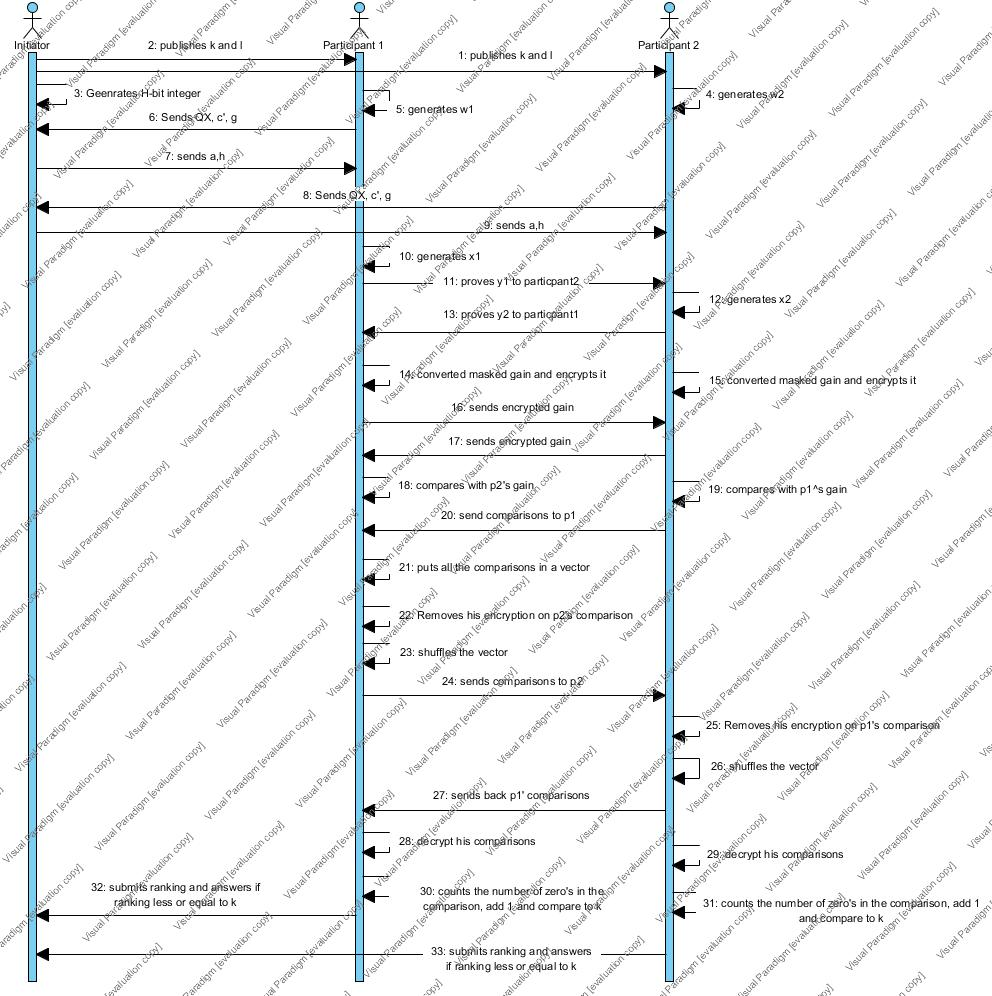
\includegraphics[width=\paperwidth]{Initator}
	\centering
\end{figure}

\chapter{Conclusion}

\paragraph{Objective:}
In this project we have analysed and implemented a secure group ranking protocol using Java programming language. 
The protocol we have studied gives the required security in the HBC model, and protects an honest participant from passive inside attacks.

\paragraph{Implementation Status:}
We need to fix the chained decryption (i.e step 9).
Furthermore, the code also needs re-factoring so that it can be used more generally as library for example. 
\paragraph{Future work}
Since it has been shown that there exist no secure distributed dot product protocol\cite{imp}. Knowing whether a dishonest initiator could learn some knowledge about the participant is a question of great interest. Unfortunately, due to time constraint the question has not  been investigated further.
\paragraph{challenges:} Choosing an implementation project was at the same time a hard choice and an interesting one. Hard because I am more versed in theoretical matters, interesting because I believe that it is a good hands-on experience. In this project, the implementation has been tedious and has required being really careful.
\paragraph{Lessons learned:} Implementation of mathematical concepts to create a cryptosystem, implementation of other various tools. Programming wise, I have come to develop more tools that helped me to be efficient and spot my mistakes faster than before. Knowledge wise, I have learned new cryptographic concepts. This includes how to securely generates a cyclic group used in cryposystems, homomorphic cryptosytems, HBC models, Zero-Knowledge proof and secure dot product protocol.\\
Finally, I would like to acknowledge Handan Kilin\c{c}, who supervised this project.

\chapter{Appendix}
\subparagraph{Proof of correctness of gain comparison.}
In this paragraph we show that the comparison algorithm used at step 7 is correct and gives the desired results.\\
Let a = $a_{l-1}...a_{1}a_{0}$ and b = $b_{l-1}...b_{1}b_{0}$ be two l bits unsigned numbers in binary form and we want to compare a to b. Let suppose W.L.O.G that the first k-1 most significant bits of a and b are the same, $0\leq k-1 \leq l$. $\gamma$ is computed computed as a bit-by-bit xor of a and b, i.e $\gamma_k = a_k \oplus b_b$. We notice here that $\gamma _v$ is always 0 for $v > k$ and  $\gamma _k$ is always 1. Let $\omega$ be a n-bits numbers where $\omega_k = (l-t+1)(1-\gamma_t)$ we notice here that $\omega _k$ is always 0. Lastly $\tau$ is a n-bits number such that $\tau_t = \omega_t + a_t$

\textbf{\textit{Case 1}}: a is smaller than b, so $a_{k} = 0 $ and $b_{k} = 1$. This implies that $\gamma^{k} = 1$. This implies that $\tau_{k}= 0 + a_{k} = 0$. 

\textbf{\textit{Case 2}}: a is greater than b. In this case $a_{k} = 1 $ and $b_{k} = 0$. This implies that that $\omega_{k} = 0$ and $\tau_{t}= 0 + a_k = 1$. 

In both cases, $\omega_{j} \geq 1$, for $j < k$. This comes form the fact that $(l-t+1)(1-\gamma _j) \geq  0$ and sum of $\gamma$'s is at least 1 due to the fact that $\gamma _k=1$. We can also see that $\omega_{j} \geq 1$, for $j > k$ since the $\omega _j$ are always 1.
As a consequence, corresponding $\tau _j \geq 1$ for $j \neq k$.  
This shows that $\tau$ will have at most one zero and will contain a zero iff a $<$ b. \\  
Now it is easy to convince ourselves that the procedure applied here for a and b is the same as the one used by the protocol expect that in the protocol the numbers are encrypted and represented as an array. 

\subparagraph{ElGamal group generation.}

Pick a prime number $q$.\\
 Take a random $p$ = $aq + 1$ until it is prime.\\
 Take a random number in $\mathbb{Z}_ p^*$ , raise it to the power $a$ modulo $p$,
and get $g$
- if $g = 1$, try again (otherwise, it must be of order $q$ in $\mathbb{Z}_p^*$ ). 

\subparagraph{Proof of correctness of masked gain.}
Let $a,b,c$ be integers such that $a > b$ and $c > 0$. let $a'=ca+c_a$ and $b'=cb+c_b $, where $c_a,c_b$ in $ \left\lbrace 0,1,..,c-1 \right\rbrace$. Is is the case that $ca - cb \geq c$. We also have that $c > c_b - c_a$. Thus $ca -cb > c_b - c_a$, finally we have $ca+c_a > cb+c_b$. This shows that the order of the partial gains are preserved by the masks
\begin{thebibliography}{9}
\bibitem{groupRank} 
Lingjun Li, Xinxin Zhao, Guoliang Xue, and Gabriel Silva. 
\textit{Privacy Preserving Group Ranking}. 
2012 32nd IEEE International Conference on Distributed Computing Systems
 
\bibitem{algo1} 
 K. Jonsson, G. Kreitz, and M. Uddin, 
\textit{``Secure multi-party sorting and ´
applications"},2011, http://eprint.iacr.org/.
\bibitem{algo2}
 M. Burkhart and X. Dimitropoulos, \textit{``Fast privacy-preserving top-k
queries using secret sharing",} in Proc. IEEE ICCCN’10, Zrich, Switzerland,
Aug. 2010.
\bibitem{algo3}
 T. Nishide and K. Ohta, \textit{``Multiparty computation for interval, equality,
and comparison without bit-decomposition protocol"}, Public Key
Cryptography–PKC 2007, pp. 343–360, 2007.
 \bibitem{algo3}
I. Damgard, M. Fitzi, E. Kiltz, J. Nielsen, and T. Toft, \textit{``Unconditionally ˚
secure constant-rounds multi-party computation for equality, comparison,
bits and exponentiation"}, Theory of Cryptography, pp. 285–304,
2006.
\bibitem{algo4}
 S. Goldwasser, S. Micali, and C. Rackoff, \textit{``The knowledge complexity
of interactive proof-systems"}, in Proc. ACM STOC’85. ACM, 1985,
pp. 291–304.
\bibitem{algo5}
I. Damgard, M. Geisler, and M. Kroigard, \textit{``Homomorphic encryption
and secure comparison"}, International Journal of Applied Cryptography,
vol. 1, no. 1, pp. 22–31, 2008.
\bibitem{algo6}
H. Lin and W. Tzeng, \textit{``An efficient solution to the millionaires problem
based on homomorphic encryption"}, in Proc. IACR ACNS. New York,
USA: Springer, 2005, pp. 456–466.
\bibitem{algo7}
P. Paillier, \textit{``Public-key cryptosystems based on composite degree residuosity
classes"}, in Proc. IACR EUROCRYPT’99, Prague, Czech Republic,
May 1999.
\bibitem{dotprod}
I. Ioannidis, A. Grama, and M. Atallah, \textit{``A secure protocol for computing
dot-products in clustered and distributed environments"}, in Proc.
IEEE ICPP’02, Vancouver, British Columbia, Aug. 2002.

\bibitem{sch}
C. Schnorr, 
\textit{``Efficient identification and signatures for smart cards"}, in
Proc. Crypto89. Springer, 1990, pp. 239–252.

\bibitem{imp}
Pedersen, Thomas Brochmann and Savaş, Erkay (2009) \textit{``Impossibility of unconditionally secure scalar products"}. Data and Knowledge Engineering, 68 (10). pp. 1059-1070. ISSN 0169-023X

\end{thebibliography}
\end{document}
